\section{Untersuchung optischer Elemente}
	
	\subsection{Methoden}
		
			\begin{figure}[ht]
				\centering
				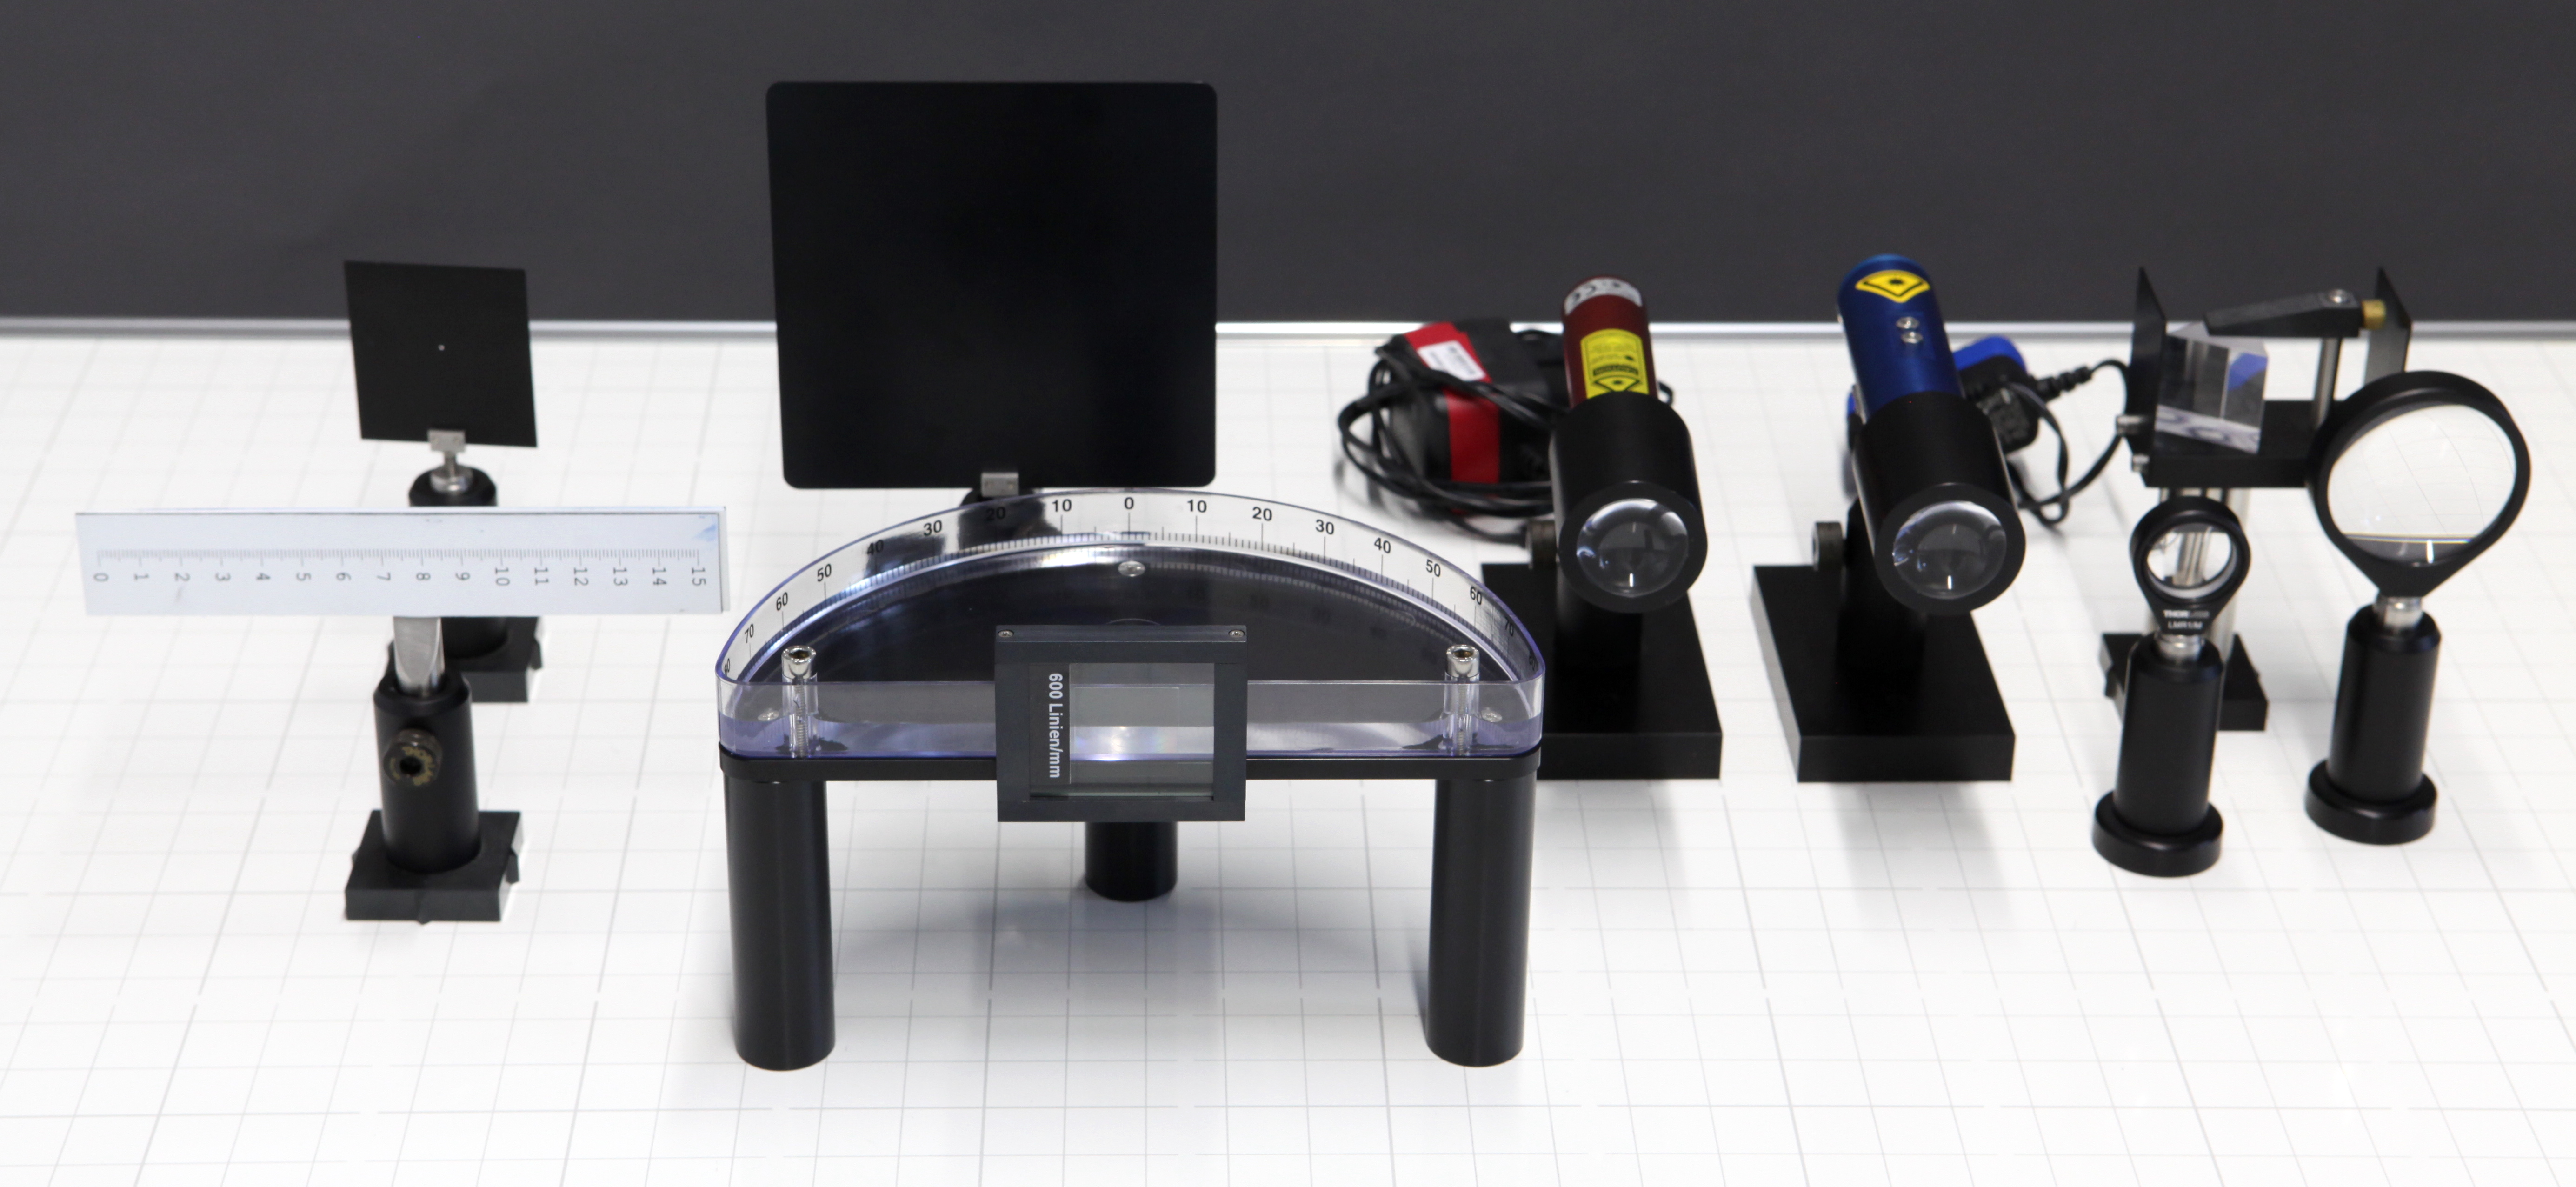
\includegraphics[width=\textwidth]{bilder/aufbau2.jpg}
			 	\caption{Für den Versuch verwendete Materialien.\cite{WWU}}
			 	\label{fig:Aufbau2}	
			\end{figure}
			Abbildung \ref{fig:Aufbau2} zeigt die für diesen Versuch verwendeten Materialien.
			Alle diese befinden sich auf einer magnetischen Unterlage, sodass diese während der Messung nicht verrutschen können.
			Zu den Materialien gehören ein roter Laser ($\lambda = \SI{650}{\nano\meter}$), ein blauer Laser ($\lambda = \SI{405}{\nano\meter}$) und eine Lochblende zur Ausrichtung eines geraden Strahlengangs, welcher parallel zu dem Raster auf der magnetischen Unterlage verlaufen soll.
			Für beide Laser soll dieser durch das Prisma und das Gitter verlaufen und für einen einzelnen durch die Linsen. % TODO ist das nicht eher durchführung (1)
			
			Das Prisma besteht aus Flintglas und besitzt von oben betrachtet die Form eines gleichseitigen Dreiecks ($\alpha = \SI{60}{\degree}$).
			Die Strahlen der beiden Laser sollen so gerichtet werden, dass sie durch den Apex des Prismas verlaufen. %TODO [1]
			Als Schirm zur Messung der Ablenkung dient die horizontal ausgerichtete Messleiste.
			Zu beobachten ist die Änderung der Ablenkung bei dem Drehen des Prismas. %TODO beobachtung [1]
			Bei symmetrischem Strahlengang ist die Ablenkung minimal.
			Aus Abstand zur Messleiste $h$ und Ablenkung $x$ von der Nulllage (keine Ablenkung) lässt sich über
			\begin{equation} \label{eq:Winkler}
				\tan \delta_m = \frac{h}{x} \Leftrightarrow \delta_m = \arctan \frac{h}{x}
			\end{equation}
			der minimale Ablenkwinkel $\delta_m$ bestimmen.
			\begin{figure}[ht]
				\centering
				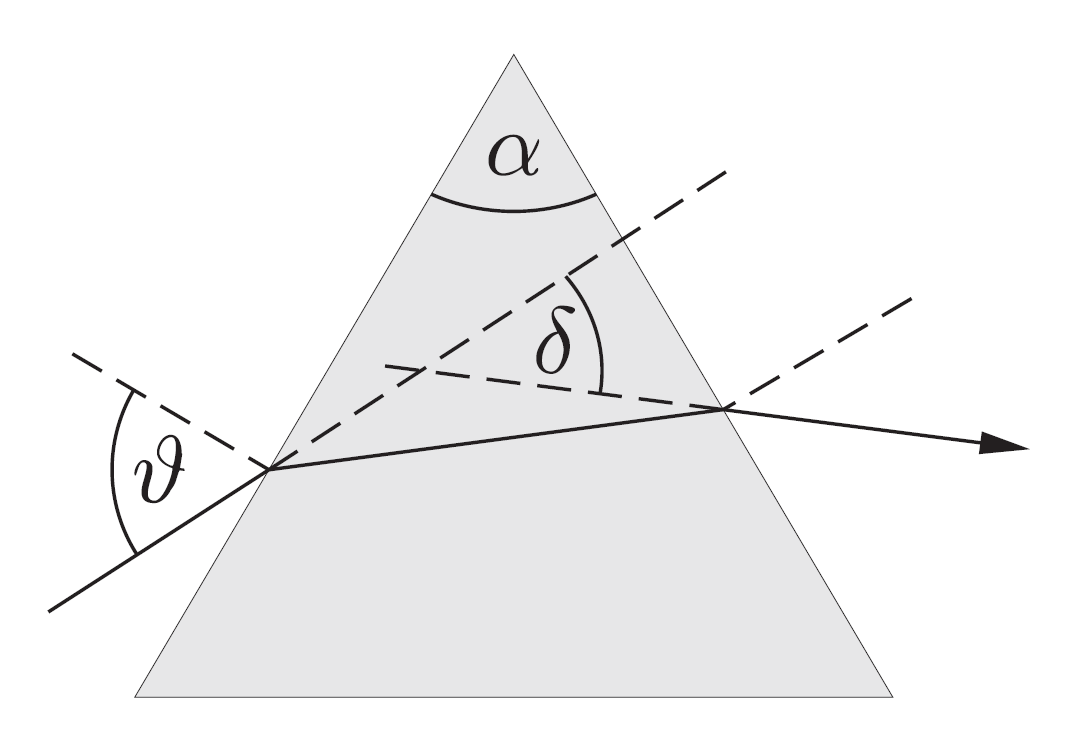
\includegraphics[width=0.5\textwidth]{bilder/prisma.png}
				\caption{Durchgang eines Lichtstrahls durch ein Prisma.\cite{WWU}}
				\label{fig:Prisma}	
			\end{figure}
			Zur Veranschaulichung dient Abb. \ref{fig:Prisma}.
			Für den symmetrischen Durchgang des Lichtstrahls durch das Prisma entfällt das $\vartheta$ in der Skizze und  es lässt sich für den Brechungsindex $n_\text{Prisma}$ des Prismas folgendes aufstellen:
			\begin{equation} \label{eq:nPrisma}
				n = \frac{\sin[(\delta_m + \alpha) / 2]}{\sin [\alpha / 2]},
			\end{equation} 
			wobei $\delta_m$ der Austrittswinkel nach dem Prisma ist.
			
			Das Gitter ist an einem offenen flachen Halbzylinder bzw. einer Halbkreisküvette angebracht, sodass die Ablenkung des Strahlengangs auf dem Gradmaß zu messen ist, welches auf der Innenseite dieser Küvette angebracht ist.
			Da diese offen ist, lässt sie sich mit einem anderem Material, hier destilliertes Wasser, füllen und daher eine andere Ablenkung des Strahls auf dem Gradmaß messen.
			An dieser Stelle lässt sich der Brechungsindex $n_\text{Wasser}$ des destillierten Wassers über das Snelliussche Brechungsgesetz $n_\text{Wasser} \sin \alpha_\text{Wasser} = n_\text{Luft} \sin \alpha_\text{Luft}$ bestimmen.
			
			Für die Linsen soll zunächst herausgefunden werden, um welche Typen es sich handelt.
			Dazu wird die Ablenkung des Laserstrahls bei den einzelnen Linsen betrachtet.
			An dieser Stelle soll zudem die Brennweite der Sammellinse bestimmt werden.
			Um diese zu bestimmen wird der Schirm verwendet und der Abstand von der Linse gesucht, bei dem alle Strahlen sich in einem Punkt treffen, auf dem Schirm der Laser also am kleinsten ist. 
			Danach sollen die Linsen so kombiniert werden, dass der Strahl vergrößert wird und dabei noch kollimiert ist.
			Hierfür ist der richtige Abstand zwischen den Linsen relevant.
			Aus diesem und der Brennweite der Sammellinse lässt sich die Brennweite der Streulinse einfach dadurch ermitteln, dass beide Brennpunkte aufeinander liegen müssen.  
			Zuletzt soll noch betrachtet werden wie sich der Strahlengang bei Verschiebung und Verkippung der Sammellinse verhält, diese also nicht ideal positioniert ist.
			Dazu wird der Strahl mit einer Strahlenaufweitung aufgeweitet um ein Flächenbild als Referenz zu haben und so den Strahlenverlauf direkt beschreiben zu können.
			Die Strahlenaufweitung wird zunächst so eingestellt, dass der Laserstrahl nach dieser kollimiert ist.
			
	\subsection{Durchführung}
		
		Angefangen wurde mit dem roten Laser.
		Dazu wurde zunächst die Lochblende verwendet um den Strahlengang parallel zu der magnetischen Unterlage auszurichten.
		In diesen Strahlengang wurde dann das Prisma und dahinter die Messleiste, in einem Abstand von $h = \SI{10+-0,58}{\centi\meter}$, gesetzt.
		Das Drehen des Prismas führte dazu, dass die Ablenkung $x$, welche auf dem Schirm größer bzw. kleiner wurde.
		Um $x = \SI{11,0+-0,03}{\centi\meter}$ auf der Messleiste veränderte sich die Ablenkung beim leichten Drehen des Prismas nur noch kaum.
		Bei dem blauen Laser mit gleichem $h$ war dies bei $x = \SI{12,2+-0,03}{\centi\meter}$ der Fall. 
		
		Für den roten Laser bei dem Gitter ergab sich eine Ablenkung von \SI{24+-0,29}{\degree} ohne destilliertem Wasser in der Küvette und \SI{15+-0,29}{\degree} mit.
		Hingegen bei dem blauen Laser \SI{18+-0,29}{\degree} ohne und \SI{11+-0,29}{\degree} mit Wasserfüllung.
		
		Da für die Linsen nur einer der Laser verwendet werden sollte, wurde dafür der rote gewählt, da dessen Lichtpunkt auf einem Schirm schärfer zu erkennen war.
		Die beiden Linsen ließen sich schnell anhand ihres Strahlengangs erkennen.
		Hält man ein Stück Papier hinter die Linse in den Strahl, so kann dieser sichtbar gemacht werden.
		Bei der größeren Linse handelt es sich um eine Sammellinse.
		Der Strahl verjüngt sich zunächst, bevor er nach dem Brennpunkt wieder auseinanderläuft.
		Bei der kleineren Linse handelt es sich um eine Streulinse, bei welcher der Strahlengang bereits direkt hinter der Linse divergiert. %TODO ist in Ordnung so?
		Der Brennpunkt der Sammellinse ließ sich bei ca. $f_\text{konvex} = \SI{12+-0,4}{\centi\meter}$ ausmachen.
		Zur Aufweitung des Strahls wurde zuerst die Streulinse vor den Laser gesetzt und der Abstand zur Sammellinse dahinter gesucht, für den der aufgeweitete Laser kollimiert war.
		Dies war bei einem Abstand von ungefähr \SI{5+-0,58}{\centi\meter} der Fall.
		
		Nachdem die Strahlenaufweitung angebracht war, zeigte sich hinter der Sammellinse wie gewohnt der Brennpunkt.
		Bei der Verschiebung der Linse läuft der Laserstrahl nun jedoch nicht mehr in der Mitte durch diese.
		Der Brennpunkt verschiebt sich ein wenig in Richtung der Linse und auf dem Schirm zeigt sich ein elliptisches Bild des Strahls.
		Nun wurde die Linse um ca. \SI{45}{\degree} vertikal verkippt, also aus dem Strahl gedreht.
		Direkt hinter der Linse bleibt der Laser scheinbar rund.
		Kurz danach jedoch fällt er in einer Achse zusammen und bildet ca. \SI{6}{\centi\meter} hinter der Linse einen vertikalen, also zur Verkippung parallelen, Strich.
		Nach ca. \SI{8{\centi\meter} fällt auch die andere Achse zusammen und bildet einen horizontalen, zur Verkippung senkrechten Strich.
		Bei größeren Abständen von der Linse ist wieder eine elliptische Verzerrung zur Kipprichtung hin zu erkennen.
		Allerdings bleibt diesmal das Bild annähernd mittig und öffnet sich bei zunehmender Verkippung zu dieser Seite hin.
		
	\subsection{Datenanalyse}
		
		Die Winkel $\delta_m$ an dem Prisma für die beiden Laser ergeben sich durch Einsetzen von $h$ und $x$ in Gleichung \ref{eq:Winkler}.
		Es ergeben sich: $\delta_{m,\text{rot}} = \SI{39,36+-1,15}{\degree}$ und $\delta_{m,\text{blau}} = \SI{42,28+-1,15}{\degree}$.
		Einsetzen dieser Werte in Gleichung \ref{eq:nPrisma} liefert die Brechungsindizes $n_\text{Prisma,rot} = \SI{1.525+-0.013}{}$ und $n_\text{Prisma,blau} = \SI{1.557+-0.013}{}$.
		
		Für den Brechungsindex des destillierten Wassers ergibt sich nach Einsetzen der gemessenen Winkel in das Snelliussche Brechungsgesetz
		\begin{equation}
			n_\text{Wasser} = n_\text{Luft} \cdot \frac{\sin \alpha_\text{Luft}}{\sin \alpha_\text{Wasser}} 
		\end{equation}
		mit $n_\text{Luft} \approx 1$ gerade $n_\text{Wasser,rot} = \SI{1.317+-0.018}{}$ für den roten Laser und $n_\text{Wasser,blau} = \SI{1.357+-0.031}{}$ für den blauen Laser.  
		
		Die Brennweite der Streulinse bestimmt sich über die Differenz der Brennweite der Sammellinse mit dem Abstand zwischen den beiden Linsen.
		Dies ergibt $f_\text{konkav} = \SI{7+-0,6}{\centi\meter}$ für die Brennweite der Streulinse.
		
		Bei Verschiebung der Sammellinse treten sphärische Abberationen auf, welche das Bild verzerren.
		Bei einer Verkippung dieser tritt hingegen Astigmatismus auf.
		
	\subsection{Diskussion}
		
		Nun stellt sich die Frage, ob die hier durchgeführten Beobachtungen und Auswertungen mit der Theorie übereinstimmen.
		Zunächst zu der Betrachtung der Brechungsindizes von dem Flintglas des Prismas, sowie des destillierten Wassers.
		Bei beiden ist zu erkennen, dass diese sich für rotes und blaues Laserlicht unterscheiden.
		Für beide ist der Brechungsindex für den roten Laser, also bei höherer Wellenlänge, kleiner als bei dem blauen Laser.
		Da es in Materie Resonanzfrequenzen gibt, ist die Phasenverschiebung und damit der Brechungsindex Frequenzabhängig.
		Diese Frequenzabhängigkeit wird Dispersion genannt.
		Die hier berechneten Werte bei dem Prisma weichen von den gegebenen\cite{WWU} von $n_\text{Prisma,rot} = \SI{1,632}{}$ um 6,5\% und von $n_\text{Prisma,blau} = \SI{1,669}{}$ um 6,7\% ab.
		Das Verhalten in Abhängigkeit der Wellenlänge stimmt an dieser Stelle zwar überein, jedoch liegen die Literaturwerte nicht annähernd in den Unsicherheiten der berechneten Werte.
		Dies könnte daran liegen, dass die Unsicherheiten die hier verwendet wurden recht genau sind (nur ca. 0,8\% des Wertes) und eher größere zu erwarten wären, weswegen eine Abweichung von ungefähr 7\% zwar eher unwahrscheinlich jedoch nicht auszuschließen wäre und auch Fehler bei dem Ablesen von $x$ nicht auszuschließen sind, da besonders der blaue Laser das Ablesen durch seine Helligkeit erschwert hat.
		Eine genaue Übereinstimmung liegt also nicht vor, jedoch verhalten sich die Werte in ihrer Abhängigkeit zumindest wie erwartet, somit sind diese Ergebnisse in keiner Weise ein Widerspruch zur Theorie.
		Für das destillierte Wasser mit Literaturwerten\cite{Refrac} von $n_\text{Wasser,rot} = \SI{1.331}{}$ und $n_\text{Wasser,blau} = \SI{1.339}{}$ liegen die Abweichungen nur bei 1,1\% für das rote Licht und 1,3\%.
		Wie zuvor liegen diese Werte nicht in den kleinen Unsicherheiten.
		Da diese Abweichungen jedoch nur um 1\% liegen, ist dennoch eine Übereinstimmung mit der Literatur zu finden.
		
		Dass die Brennweiten der Linsen mit der verwendeten Methode bestimmt werden konnten, zeigt zumindest, dass es möglich ist diese so zu bestimmen, jedoch auch sehr ungenau ist.
		Die Beobachtungen bei dem aufgeweiteten Strahl, das Näherrücken des Brennpunkts an die Linse, bei dem Drehen dieser bzw. bei dem Durchgang des Strahls durch den Rand der Linse deutet auf eine sphärische Aberration, ein Linsenfehler der diesen Effekt im Wesentlichen erklärt.
		Bei den Beobachtung beim Neigen der Linse hingegen werden durch einen anderen Linsenfehler, den Astigmatismus erklärt.
		Dieser besagt, das schräg durch die Linse tretende Lichtbündel kein Bild mehr, sondern zwei Bildlinien erzeugen.
		
		Somit lassen sich die Beobachtungen und Auswertungen alle durch die Theorie erklären, wenn auch die Abweichungen von den Literaturwerten bei dem Prisma ein wenig höher liegen.